\section{Systemarkitektur}
\label{chap:systemarkitektur}

Domain modellen anvendes som en overgang mellem kravspecifikation og systemarkitektur.
I kravspecifikation beskrives hvad der sker ved interaktion med systemet. Mens
systemarkitekturen bruges til at beskrive systemet i blokke og til at skitsere både interne
og eksterne forbindelser. Domain modellen bruges til at beskrive hele systemets domæne.
Der kigges ikke på hardware vs. software, der kigges i stedet på "enheder"og deres
ansvarsområder.\\

\begin{figure}[H]
	\centering
	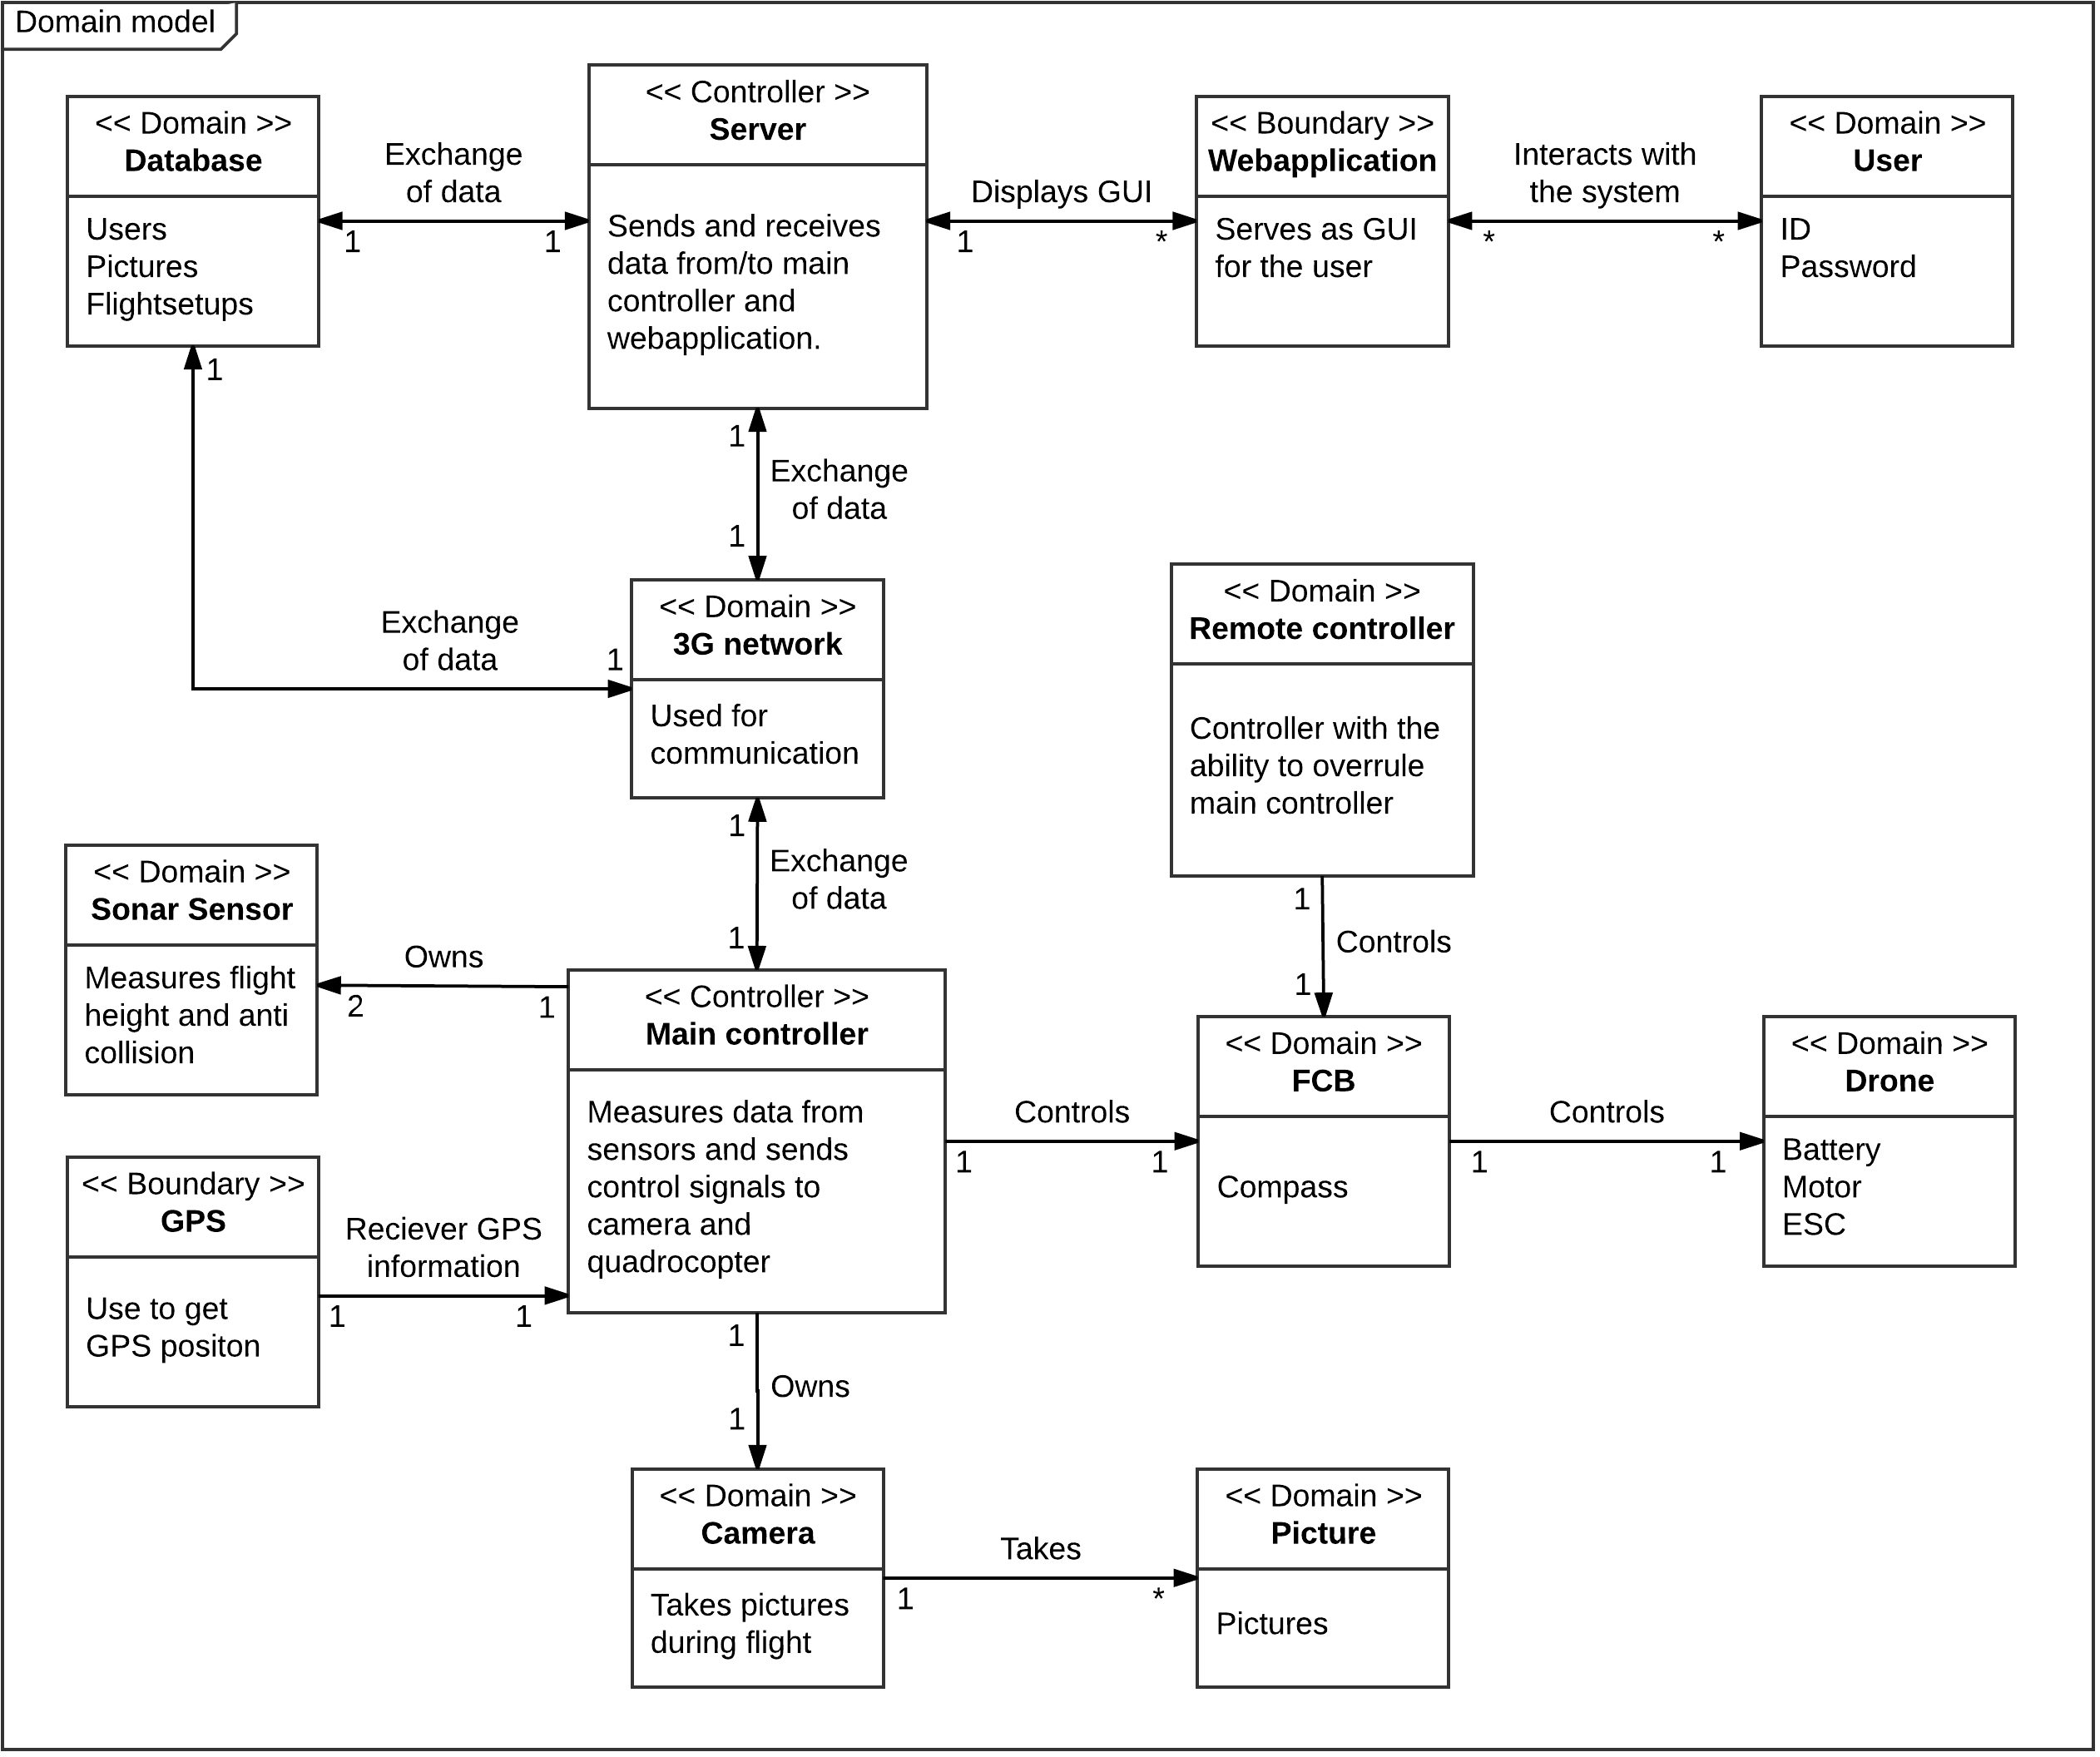
\includegraphics[width=1\textwidth]{Billeder/domain_model.png}
	\caption{Domain model}
	\label{fig:domain}
\end{figure}


\newpage

Efter at have udarbejdet kravspecifikation, systemskitse og domain model, var der formet en ide om hvordan systemet skulle fungere. I det følgende beskrives hvordan systemarkitekturen er udformet. 


Systemarkitekturen er udført ved brug af SysML og UML diagrammer. 
SysML bruges til beskrivelse af systemets hardware i blokke og som samlet system. Ud fra N + 1 og applikations modellen udformes UML diagrammer, der bruges til beskrivelse af systemets software. 
Foruden SysML og UML diagrammer benyttes en række andre diagrammer, i det følgende beskrives nogle af de mest centrale diagrammer.\\


\textbf{Use case}\\
Use cases og tilhørende diagrammer er benyttet i projektforløbets indledende faser. De bruges til at definere systemets kunnen og opdele systemet i mindre dele. Use cases har i høj grad fungeret som et omdrejningspunkt, hvorfra alt funktionalitet udspringer.


\textbf{SysML}\\
Der er benyttet to slags SysML diagrammer til dokumentation af systemets hardware. Block definition diagrammer (bdd'er) er brugt til at identificere og beskrive systemets hardware blokke og deres indbyrdes forhold. Internal block diagrammer (ibd'er) er brugt til at vise de identificerede blokkes interne og eksterne forbindelse, hvordan blokkene kommunikerer og hvilke signaler der flyder imellem dem.


\textbf{UML}\\
På baggrund af use cases og domain modellen udformes pakkediagrammer, der bruges til at beskrive ansvarsområder i systemet. Sekvensdiagrammer bruges til at identificere systemets klasser, klassernes metoder samt timing i systemet. Klasser samt tilhørende metoder og attributter beskrives ved hjælp af klassediagrammer. State machines bruges til at beskrive flow mellem forskellige states. 


\newpage

\subsection{Hardware}
I dette afsnit beskrives hvordan systemets hardwarearkitektur er udformet vha. SysML diagrammer. Indledningsvis bruges block definition diagrammer til at identificere og beskrive systemets blokke. Senere åbnes udvalgte blokke og de interne og eksterne forbindelser vises med internal block diagrammer. 


\subsubsection*{Block definition diagram}

Det overordnede bdd på figur \ref{fig:bdd_asd} viser hvilke hardware blokke systemet består af, samt hvilke parts blokkene indeholder.

\begin{figure}[H]
	\centering
	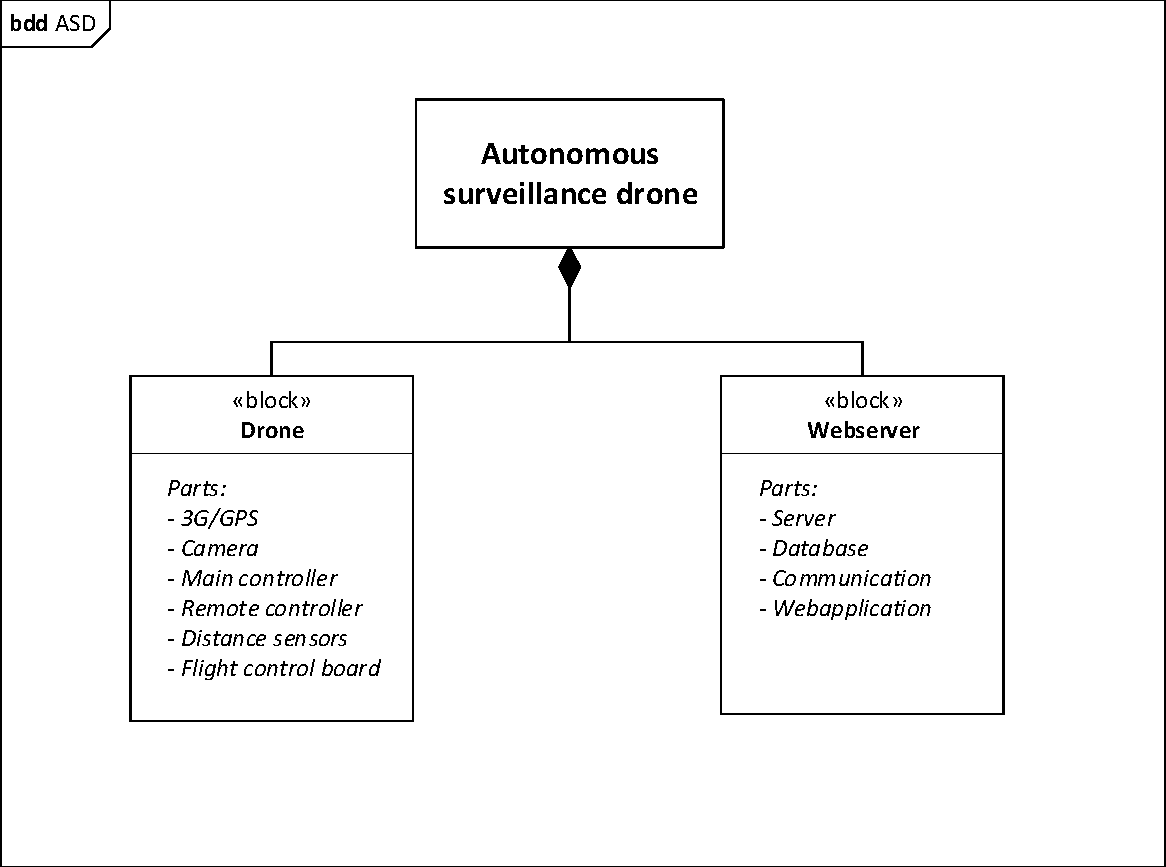
\includegraphics[width=1.0\textwidth]{Billeder/Projektbeskrivelse/bdd_overordnet.pdf}
	\caption{Overordnet bdd for systemet}
	\label{fig:bdd_asd}
\end{figure}

\textbf{Drone} \\
Drone blokken indeholder alle de hardwareenheder der giver funktionalitet til drone. Beskrivelse af de eksterne og interne forbindelser mellem de forskellige parts er beskrevet nærmere med ibd'er.

\textbf{Webserver} \\
Webserver blokken indeholder server, database, communication og webapplikationen.

\newpage

\subsubsection*{Internal block diagram}
\vspace{-0.3cm}	

På figur \ref{fig:ibd_asd} vises et overordnet ibd for systemet. ibd'et beskriver hvordan systemets største blokke kommunikerer med hinanden og omverden. Desuden beskriver ibd'et hvilken type signaler der anvendes. 

\begin{figure}[H]
	\centering
	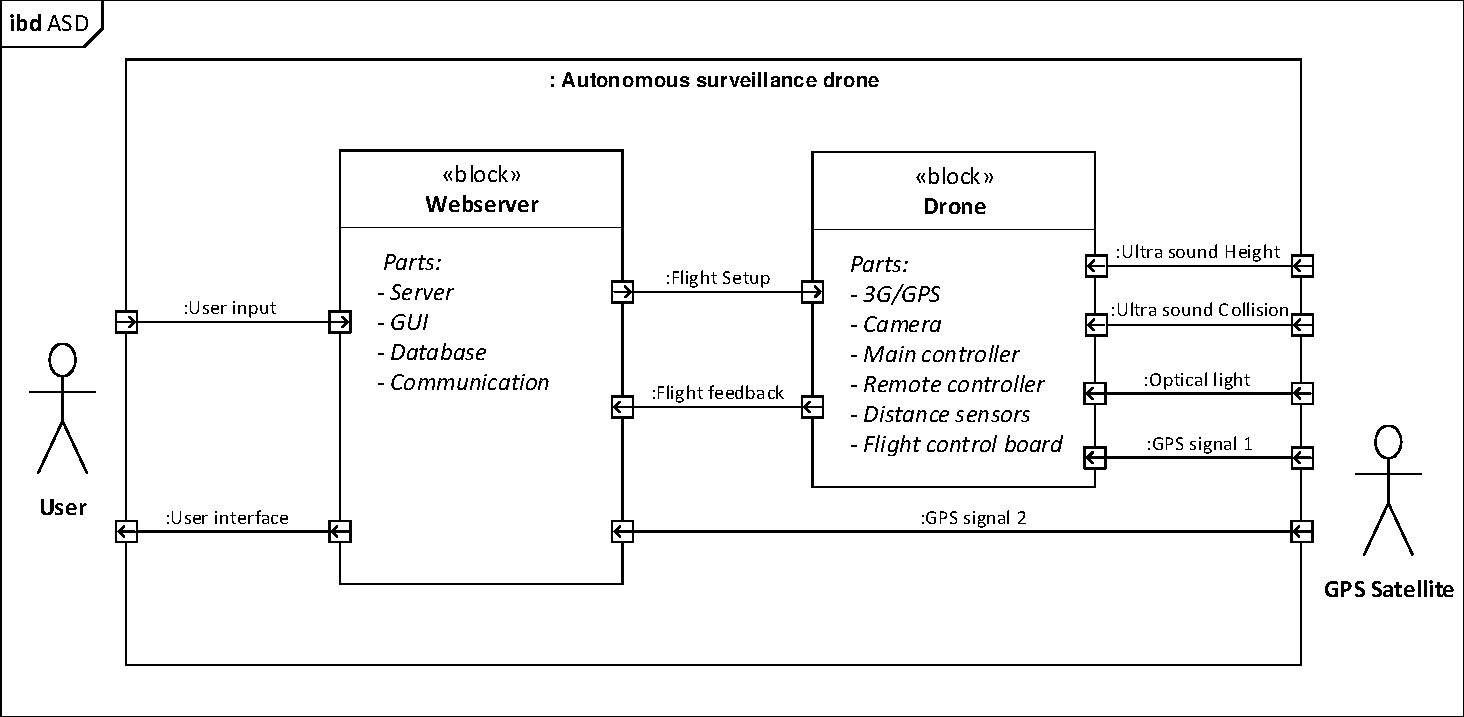
\includegraphics[width=1\textwidth]{Billeder/Projektbeskrivelse/ibd1_overordnet.pdf}
	\caption{Overordnet ibd for systemet}
	\label{fig:ibd_asd}
\end{figure}

Da drone blokken er stor og indeholder mange part kræves yderlige beskrivelse. På den følgende side åbnes drone blokken og de internal forbindelse vises.

\newpage


På figur \ref{fig:ibd_drone} vises et ibd, der går mere i dybden med drone blokken. ibd'et åbner drone blokken og viser hvordan parts i drone blokken kommunikerer med hinanden. 

\begin{figure}[H]
	\centering
	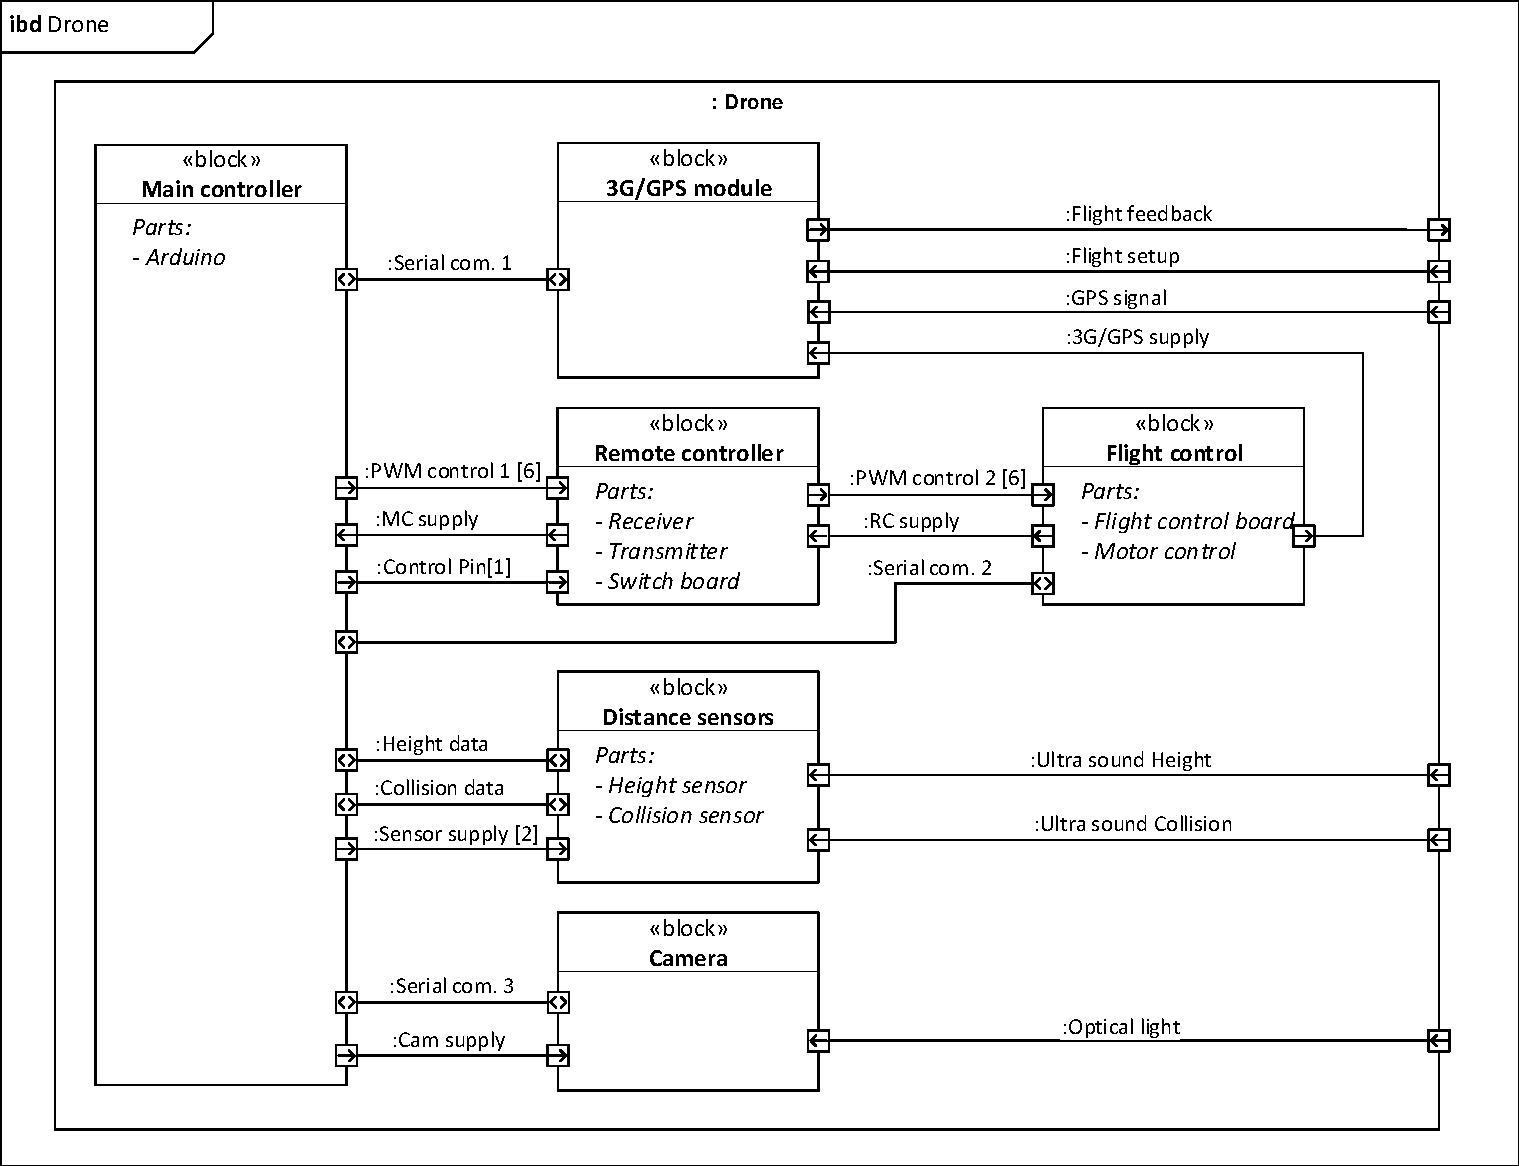
\includegraphics[width=1\textwidth]{Billeder/Projektbeskrivelse/ibd2_drone.pdf}
	\caption{ibd drone}
	\label{fig:ibd_drone}
\end{figure}


For yderlige beskrivelser af parts fra drone blokken henvises til ibd'er i hardwarearkitektur [X].
Der vises ikke udvidede ibd'er for webserver, da webserver ikke indeholder hardware og derfor beskrives nærmere ved brug af UML diagrammer i software afsnittet.



\newpage

\subsection{Software}

I dette afsnit beskrives hvordan softwarearkitekturen ved brug af N+1 og applikations modellen tager udgangspunkt i use cases og ender ud i detaljerede klassedigrammer. 
   
\subsubsection*{Pakkediagrammer}
\vspace{-0.3cm}	
Indledningsvis identificeres pakkediagrammer ud fra use cases og domain modellen. På figur \ref{fig:package_drone} vises et pakkediagram tilhørende dronens software. Pakkerne i pakkediagrammet bruges til at definere de forskellige ansvarsområder i systemts software. For nærmere beskrivelser af pakkediagrammer over systemets software henvises til logical view [X].
 
\begin{figure}[H]
	\centering
	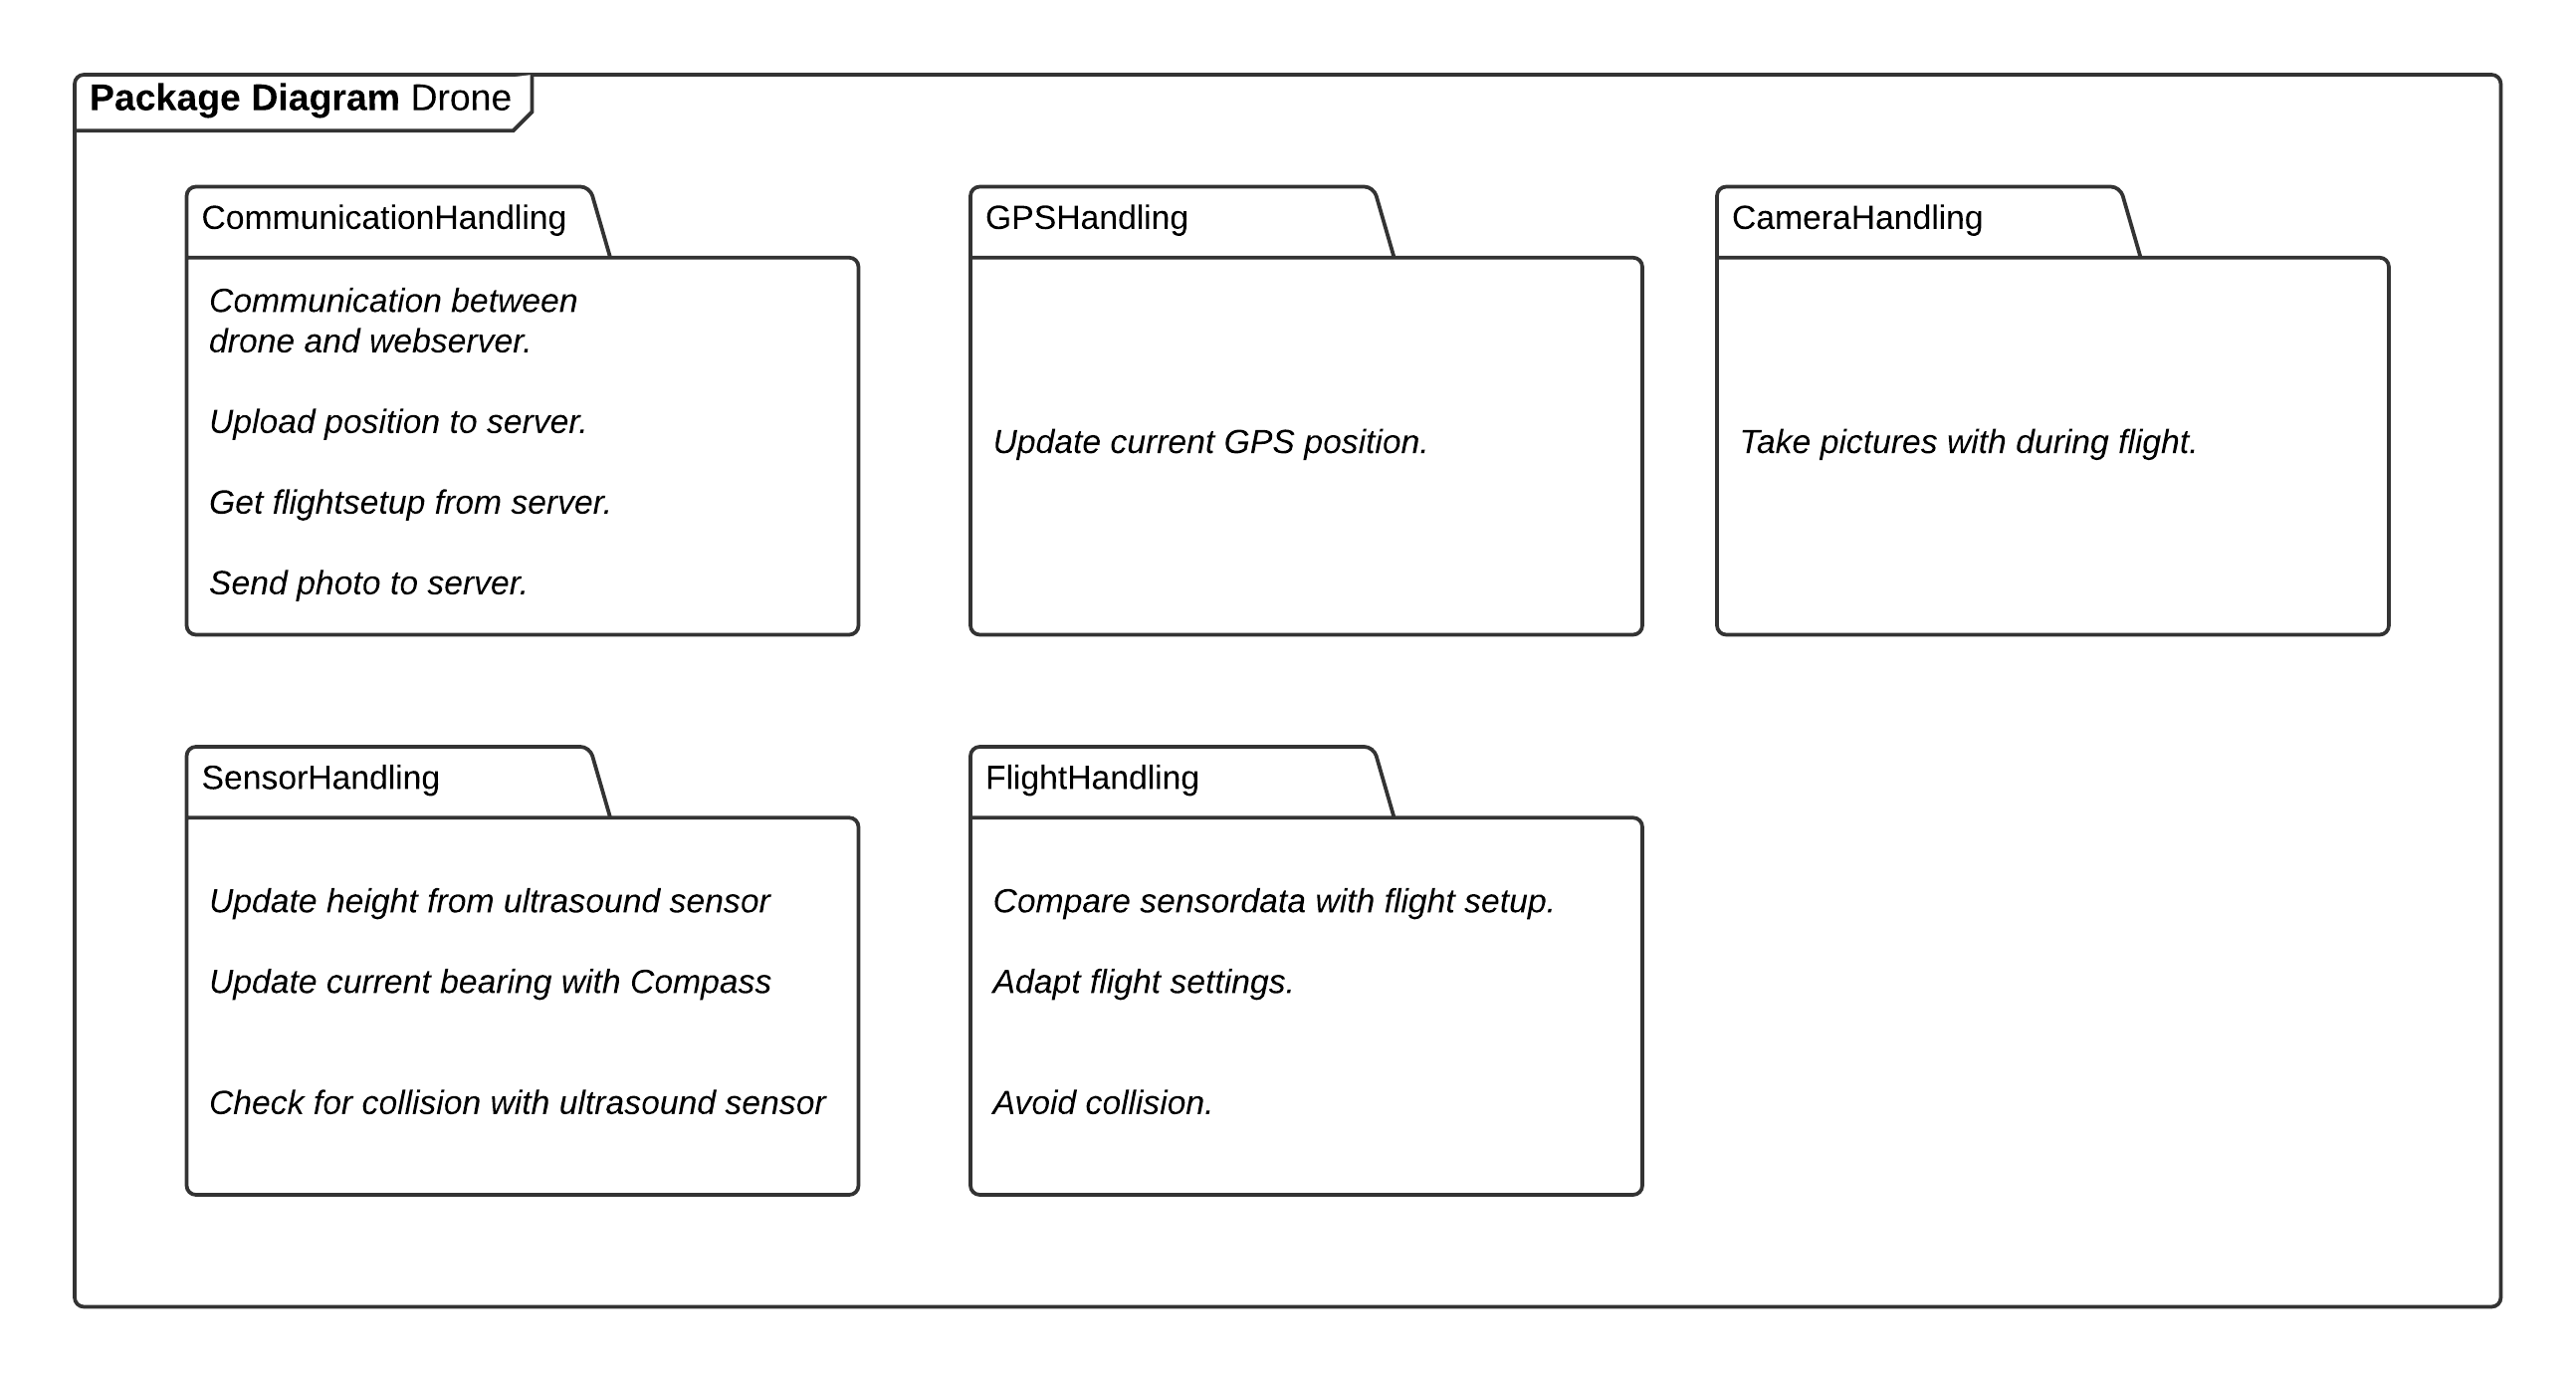
\includegraphics[width=1\textwidth]{Billeder/Projektbeskrivelse/Packagediagram_drone}
	\vspace{-0.9cm}	
	\caption{Overordnet pakkediagram for drone}
	\label{fig:package_drone}
\end{figure}

\newpage

\subsubsection*{Sekvensdiagrammer}
\vspace{-0.3cm}	

Efter at have udformet pakkediagrammer påbegyndes udformning af sekvensdiagrammer. Disse diagrammer bruges til at identificere softwareklasser, klassernes metoder, klassernes indbyrdes forhold, samt timing i systemet. Enheder der indgår i sekvensdiagrammerne tages ud fra domain modellen. 

Sekvensdiagrammet på figur \ref{fig:login_flysetting} viser et eksempel på en use case omsat til et sekvensdiagram. Sekvensdiagrammet bruges til overordnet at vise hvordan bruger interagerer med webapplikation når der laves ny flyveopsætning. For yderlige beskrivelser af sekvensdiagrammer tilhørende systemet henvises til logical view [X].

 
\begin{figure}[H]
	\centering
	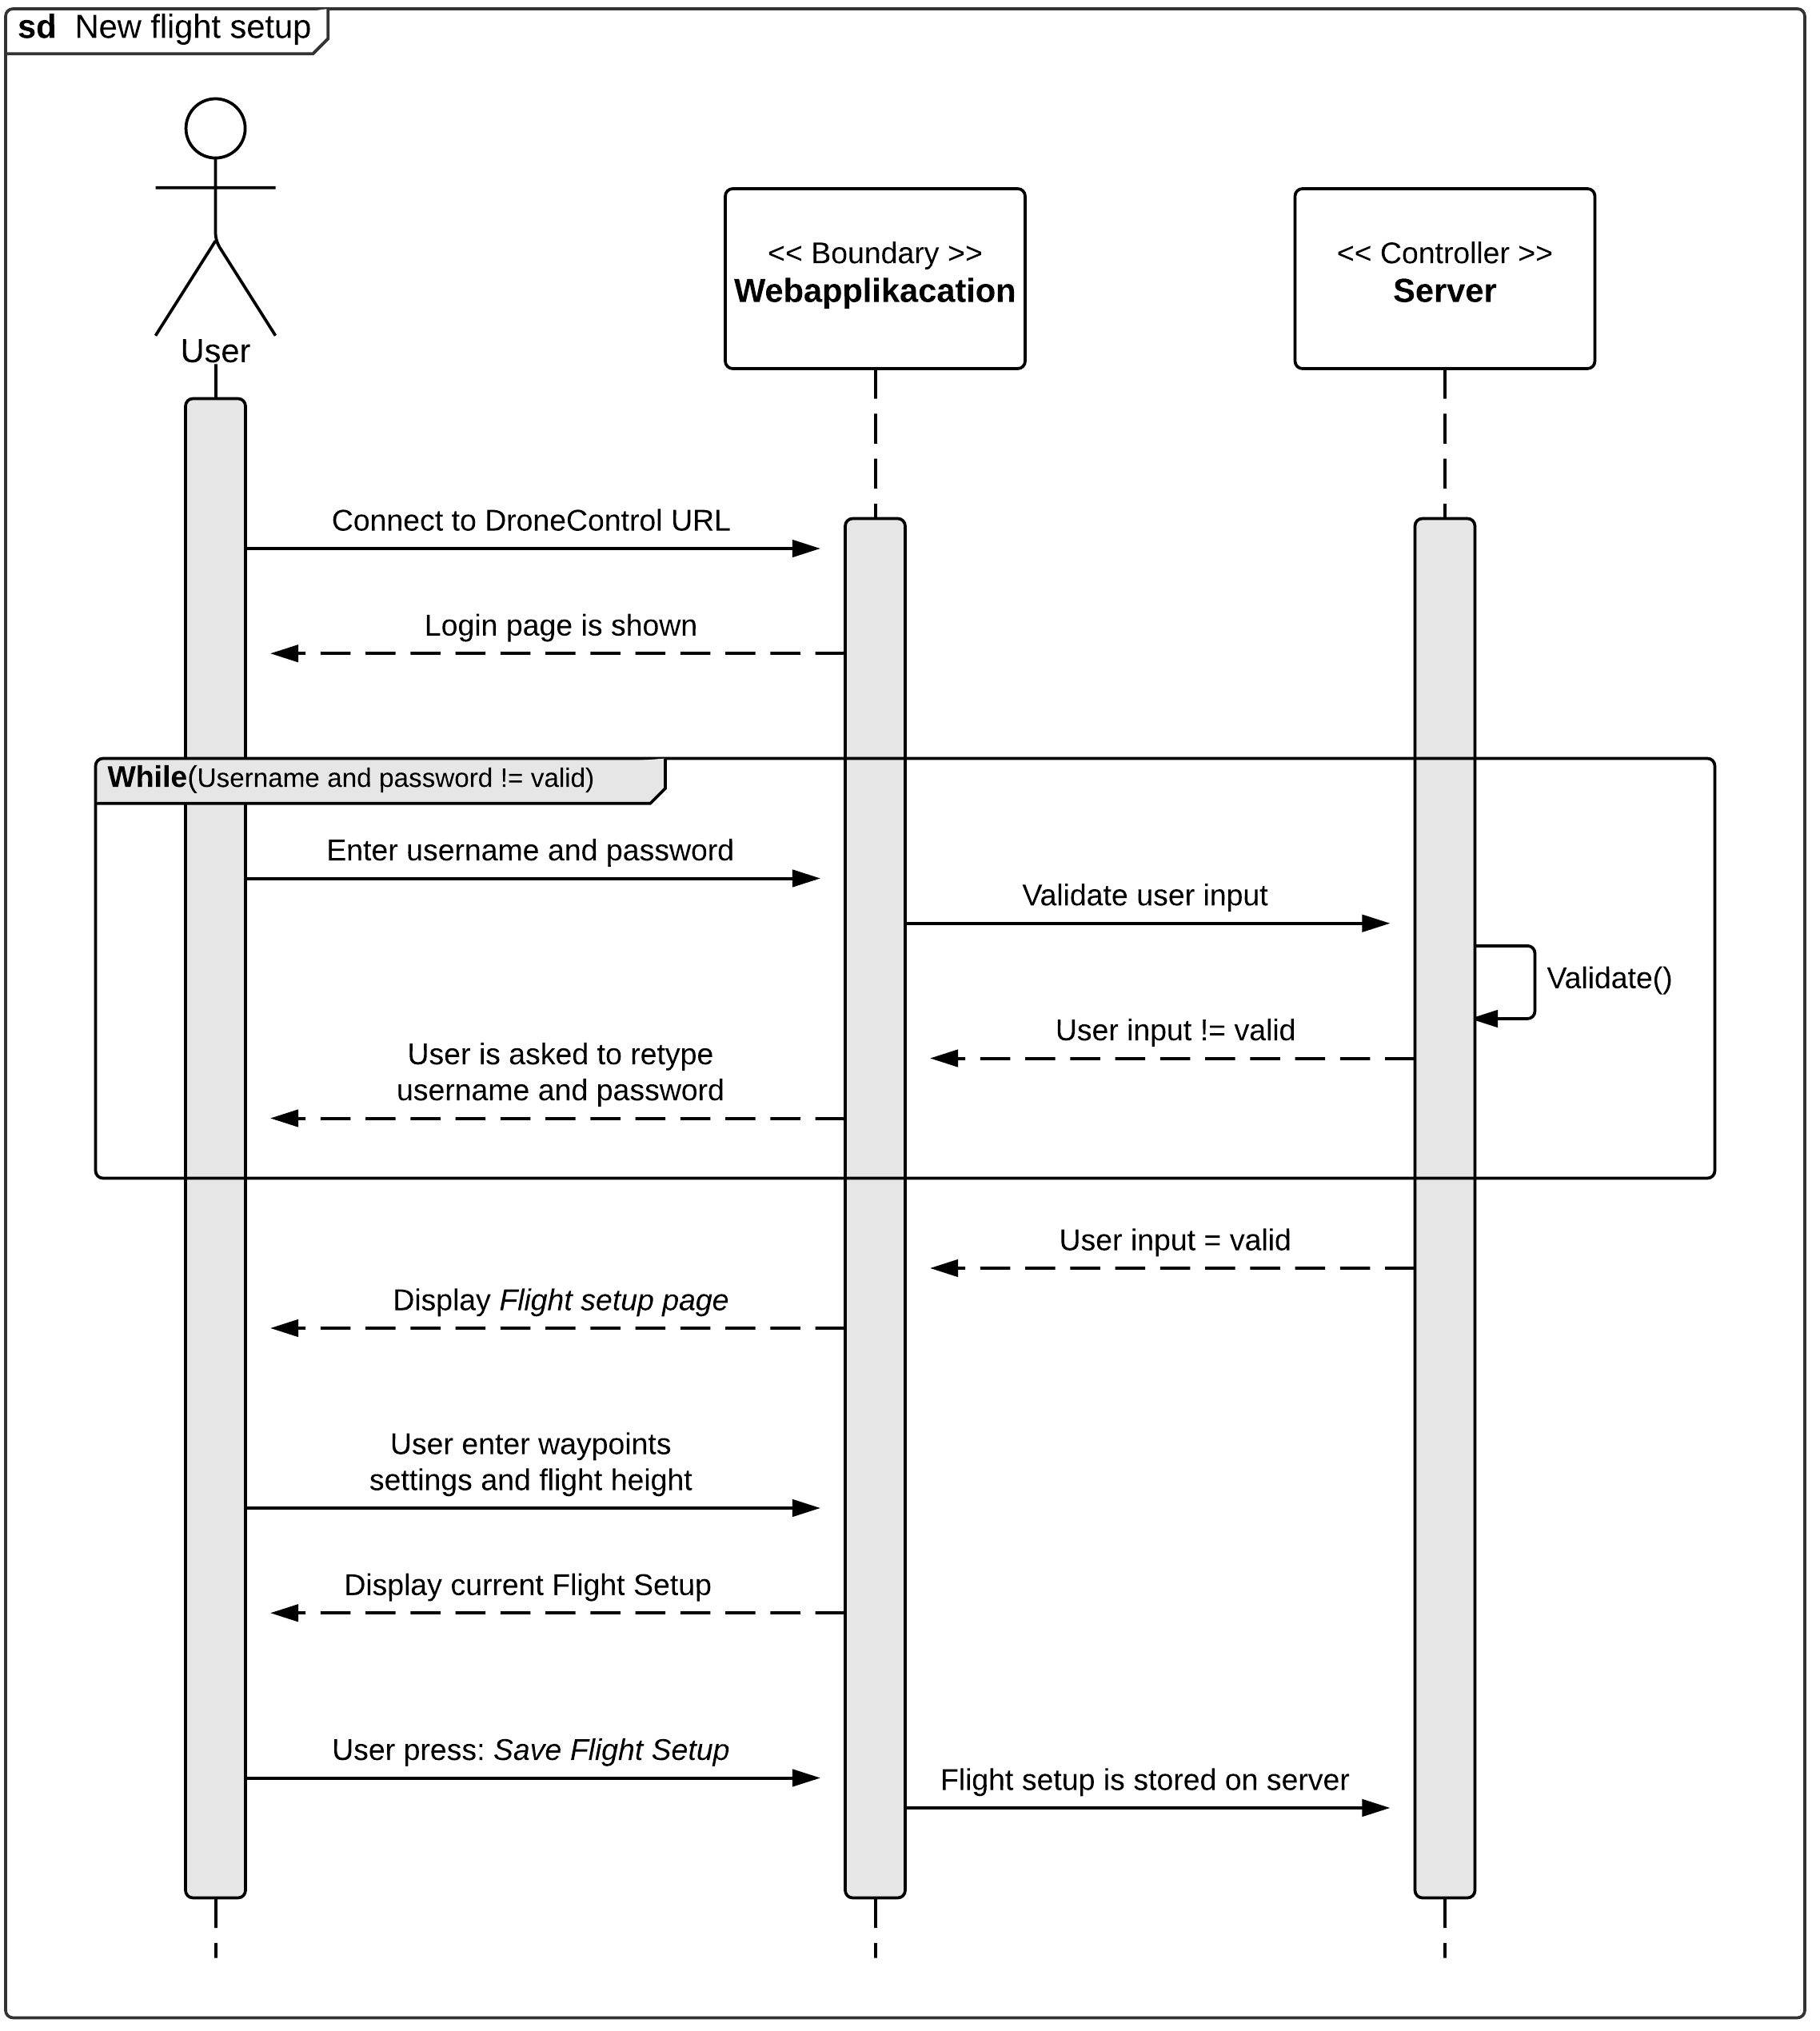
\includegraphics[width=1\textwidth]{Billeder/sekvens.png}
	\vspace{-0.6cm}	
	\caption{Sekvensdiagram - ny flyveopsætning}
	\label{fig:login_flysetting}
\end{figure}

\newpage
\subsubsection*{Klassediagrammer}
\vspace{-0.3cm}	

Efter at have udformet sekvensdiagrammer er der opbygget et vist kendskab til de forskellige klasser, deres metoder og deres indbyrdes forhold. For på overskuelig vis at illustrere og beskrive systemets softwareklasser laves klassediagrammer.

På figur \ref{fig:class_drone} vises et klassediagram tilhørende dronens software. Bemærk at klassediagrammet er fra første iteration, hvilket betyder det er relativt lille og ikke indeholder så mange klasser og metoder.

For mere information om de enkelte klasser og deres ansvarsområder henvises til logical view [x].

\begin{figure}[H]
	\centering
	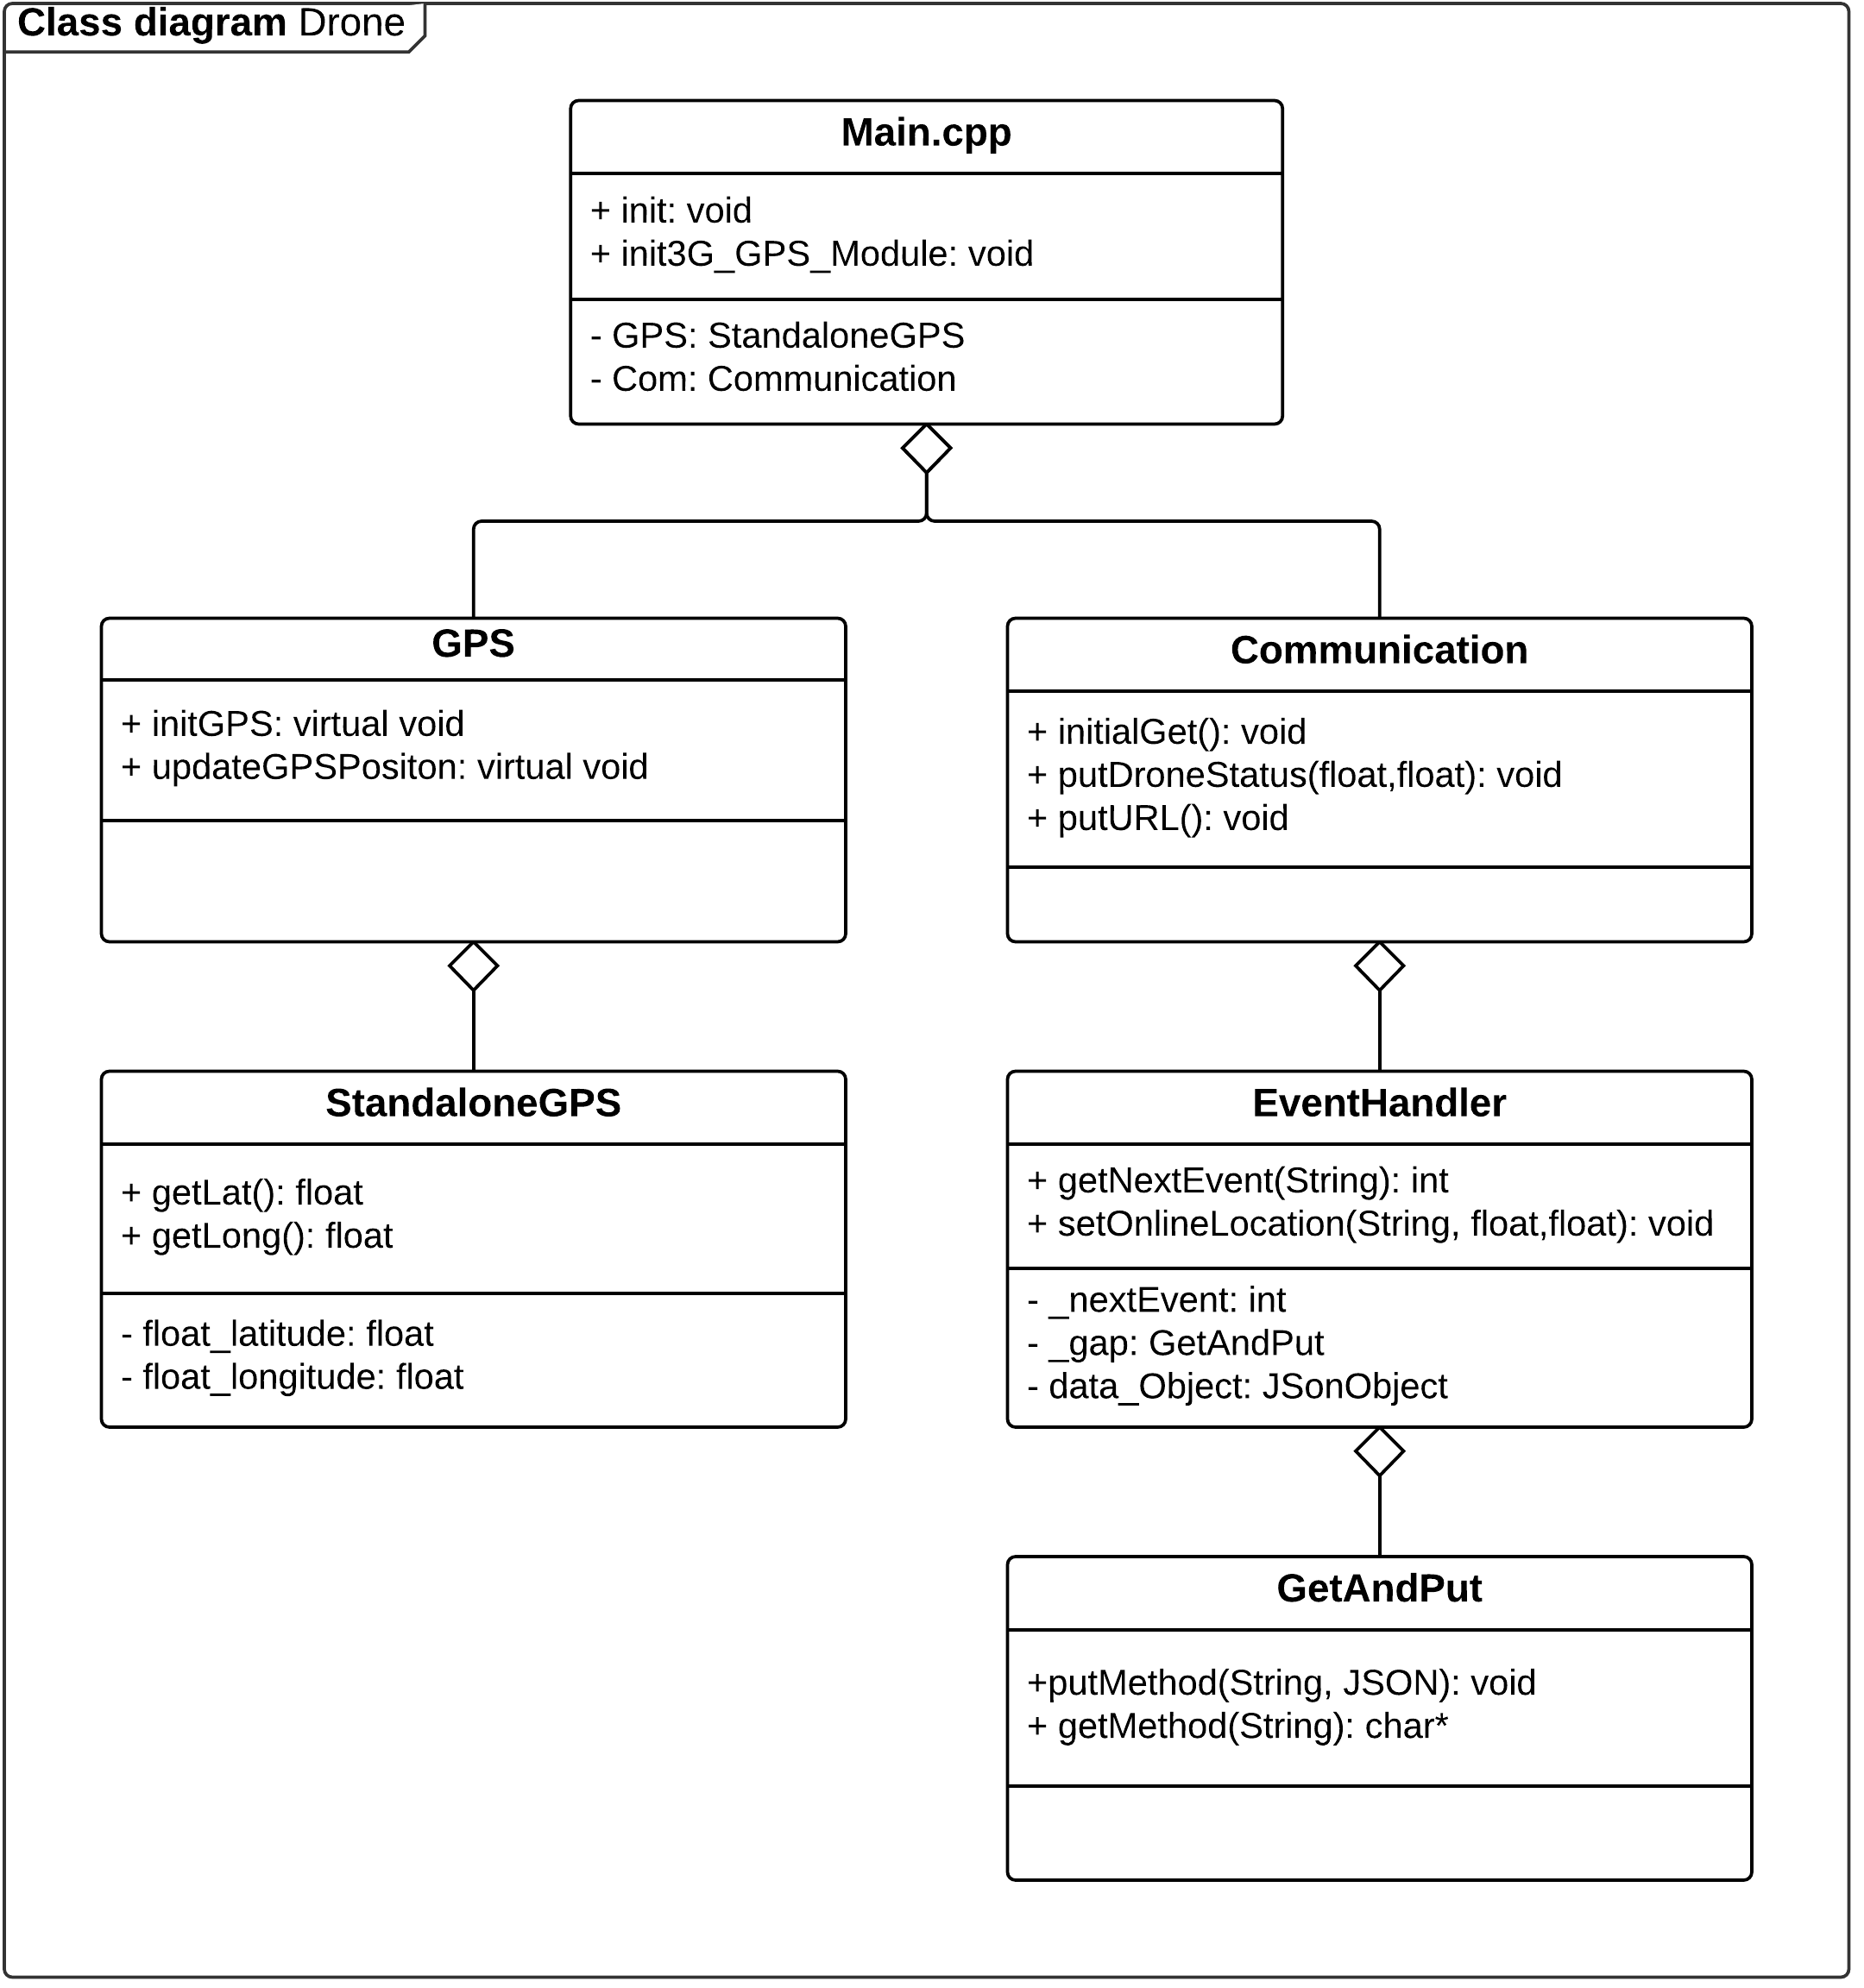
\includegraphics[width=1\textwidth]{Billeder/classdiagram.png}
	\vspace{-0.6cm}	
	\caption{Klassediagram drone}
	\label{fig:class_drone}

\end{figure}
